\documentclass[border=3pt]{standalone}
\usepackage{amsmath,amssymb}
\usepackage{tikz}
\usetikzlibrary{arrows.meta,positioning,shapes.geometric}
% Section 2 flowchart: which symmetry reductions apply to a tournament T and a base B (his request,
% 2026-10-18).  Hand-written: there is no data to check, only the logic of Section 2.1.
\begin{document}
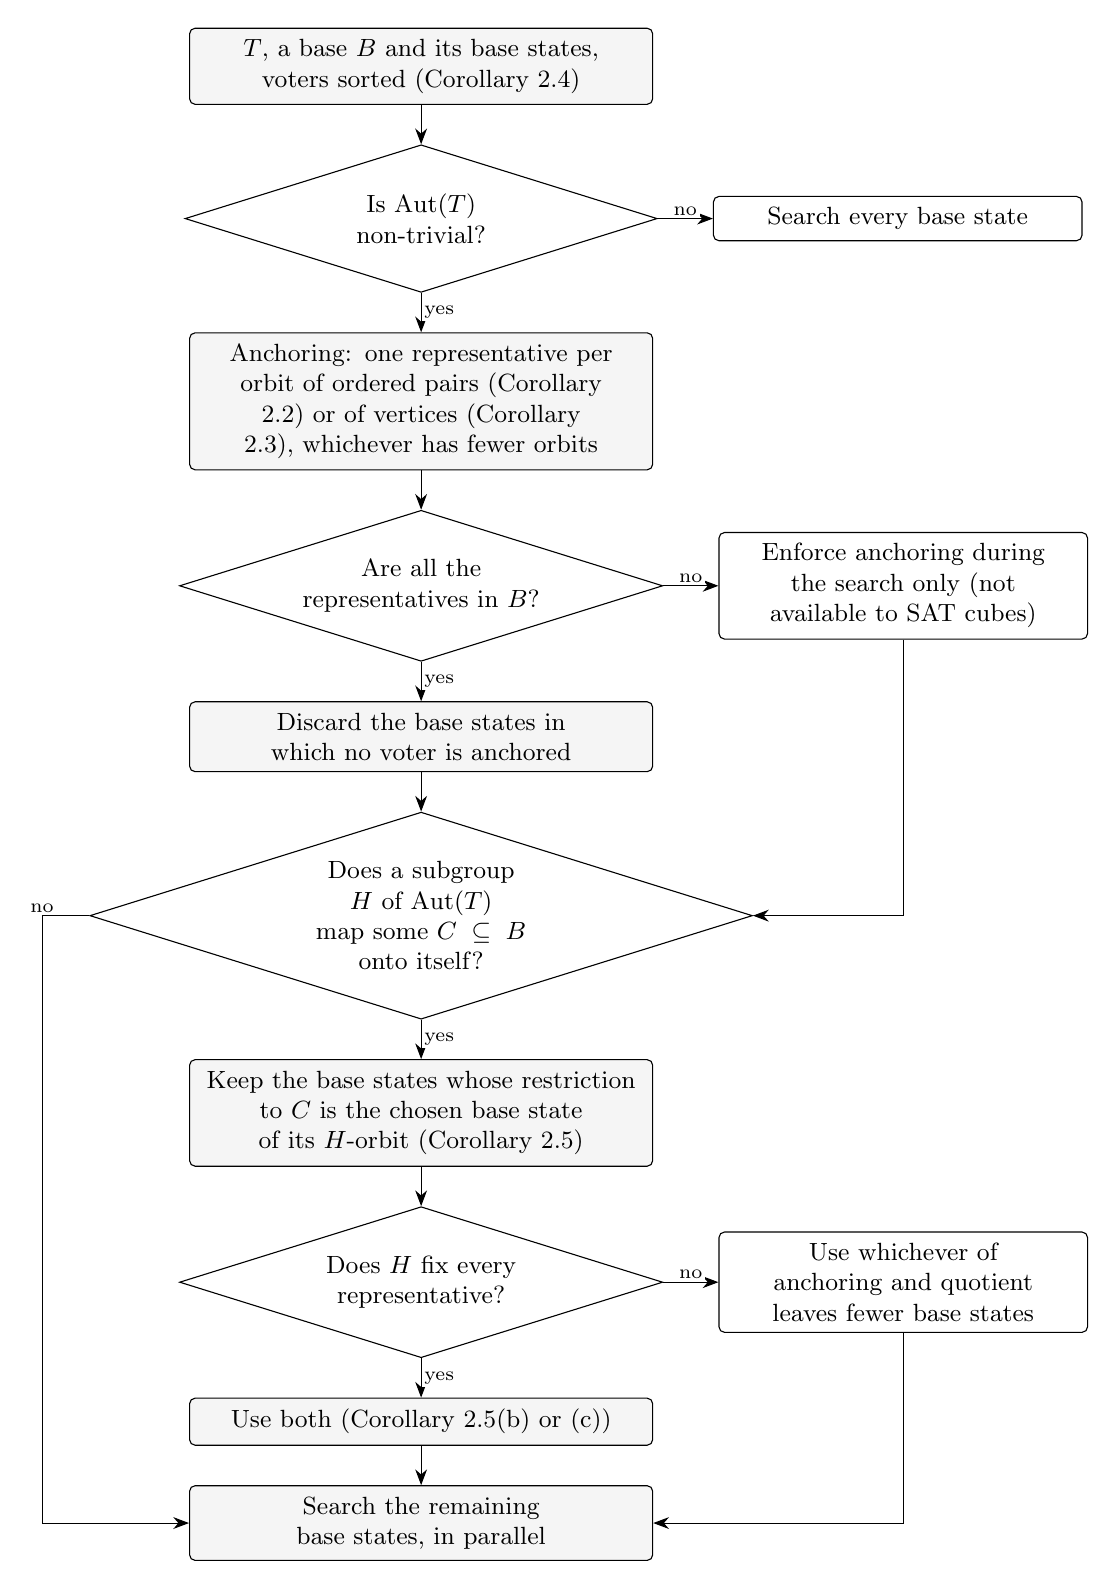
\begin{tikzpicture}[
  font=\small, node distance=5mm and 7mm, execute at begin node={\hyphenpenalty=10000\exhyphenpenalty=10000}, >={Stealth[length=2mm]},
  act/.style={draw, rounded corners=2pt, align=center, text width=56mm, inner sep=4pt, fill=black!4},
  q/.style={draw, diamond, aspect=3.2, align=center, inner sep=0pt, text width=40mm},
  side/.style={draw, rounded corners=2pt, align=center, text width=44mm, inner sep=4pt},
  lab/.style={font=\scriptsize, fill=white, inner sep=1pt}]
\node[act] (in) {$T$, a base $B$ and its base states,\\voters sorted (Corollary 2.4)};
\node[q, below=of in] (aut) {Is $\mathrm{Aut}(T)$\\non-trivial?};
\node[side, right=of aut] (none) {Search every base state};
\node[act, below=of aut] (anc) {Anchoring: one representative per orbit of ordered pairs (Corollary 2.2)
  or of vertices (Corollary 2.3), whichever has fewer orbits};
\node[q, below=of anc] (inb) {Are all the\\representatives in $B$?};
\node[side, right=of inb] (dfs) {Enforce anchoring during the search only (not available to SAT cubes)};
\node[act, below=of inb] (filt) {Discard the base states in which no voter is anchored};
\node[q, below=of filt] (sub) {Does a subgroup $H$ of $\mathrm{Aut}(T)$\\map some $C \subseteq B$ onto itself?};
\node[act, below=of sub] (quo) {Keep the base states whose restriction to $C$ is the chosen base state
  of its $H$-orbit (Corollary 2.5)};
\node[q, below=of quo] (fix) {Does $H$ fix every\\representative?};
\node[side, right=of fix] (pick) {Use whichever of anchoring and quotient leaves fewer base states};
\node[act, below=of fix] (both) {Use both (Corollary 2.5(b) or (c))};
\node[act, below=of both] (run) {Search the remaining base states, in parallel};
\draw[->] (in) -- (aut);
\draw[->] (aut) -- node[lab, above] {no} (none);
\draw[->] (aut) -- node[lab, right] {yes} (anc);
\draw[->] (anc) -- (inb);
\draw[->] (inb) -- node[lab, above] {no} (dfs);
\draw[->] (inb) -- node[lab, right] {yes} (filt);
\draw[->] (filt) -- (sub);
\draw[->] (dfs.south) |- (sub.east);
\draw[->] (sub) -- node[lab, right] {yes} (quo);
\draw[->] (sub.west) -- ++(-6mm,0) node[lab, above] {no} |- (run.west);
\draw[->] (quo) -- (fix);
\draw[->] (fix) -- node[lab, above] {no} (pick);
\draw[->] (fix) -- node[lab, right] {yes} (both);
\draw[->] (both) -- (run);
\draw[->] (pick.south) |- (run.east);
\end{tikzpicture}
\end{document}
